%%%%%%%%%%%%%%%%%%%%%%%%%%%%%%%%%%%%%%%%%%%%
\section{Why Movement Variability?}


{
%\paper{
%Bernstein 1967 in \textbf{The co-ordination and regulation of movements};
%}
\begin{frame}[fragile]{Few challenges when quantifying movement variability}
  \begin{columns}
   

 \begin{column}{.3\linewidth}
    
	\textbf{Theoretical challenges}
  \begin{itemize}
        \item Modelling human movement (tasks, environments, agent, perception, action)
        \item Modelling human variability (complexity vs predictability)
        \item ?
      \end{itemize}
    \end{column}

   \begin{column}{.3\linewidth}
	
	\textbf{Choosing the right tools} 
           \begin{itemize}
                \item Time-based domain,
		\item Frequency-based domain
		\item Nonlinear dynamics
                \item ?
              \end{itemize}
	\end{column}

   \begin{column}{.3\linewidth}
	\textbf{Technical challenges}
           \begin{itemize}
                \item non-stationarity, 
		\item non-linearity, 
		\item data length, 
		\item sensor source, 
		\item noise,
                \item ?
              \end{itemize}
	\end{column}



  \end{columns}


\end{frame}
}



%%%%%%%%%%%%%%%%%%%%%%%%%%%%%%%%%%%%%%%%%%%%%%%%%%%%%%%%
{
\paper{
Bernstein 1967 in \textbf{The co-ordination and regulation of movements};
Newell and Vaillancourt 2001 in \textbf{Hum Mov Sci};
Davids et al. 2003 in \textbf{Sport Medicine};
Warren 2006 in \textbf{Psychological Review}
}
\begin{frame}{Modeling Human Movement}
    \begin{figure}
        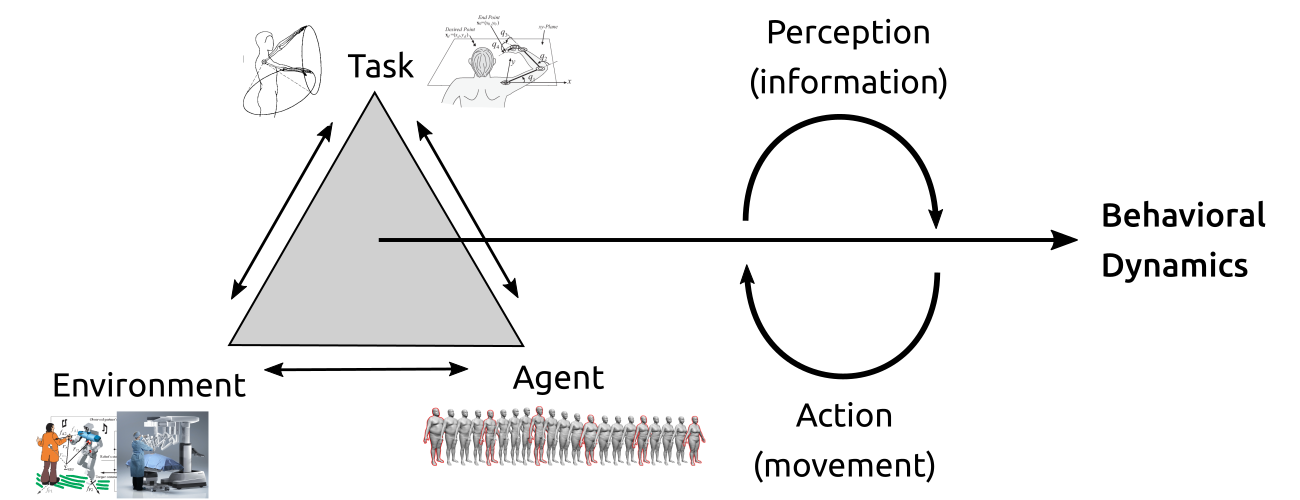
\includegraphics[width=1.0\linewidth]{./figs/modeling-movement/versions/drawing-v01.png}
	%\caption{Newell's model of movement constrains} 
   \end{figure}
\end{frame}
}



%%%%%%%%%%%%%%%%%%%%%%%%%%%%%%%%%%%%%%%%%%%%%%%%%%%%%%%%
{
\paper{
Stergiou et al. 2006 in {\bf Neurologic Physical Therapy};
Stergiou and Decker 2011 in {\bf Human Movement Science};
Tononi et al. 1998 in {\bf Trends in Cognitive Sciences}
}
\begin{frame}{Modelling Movement Variability}
    \begin{figure}
        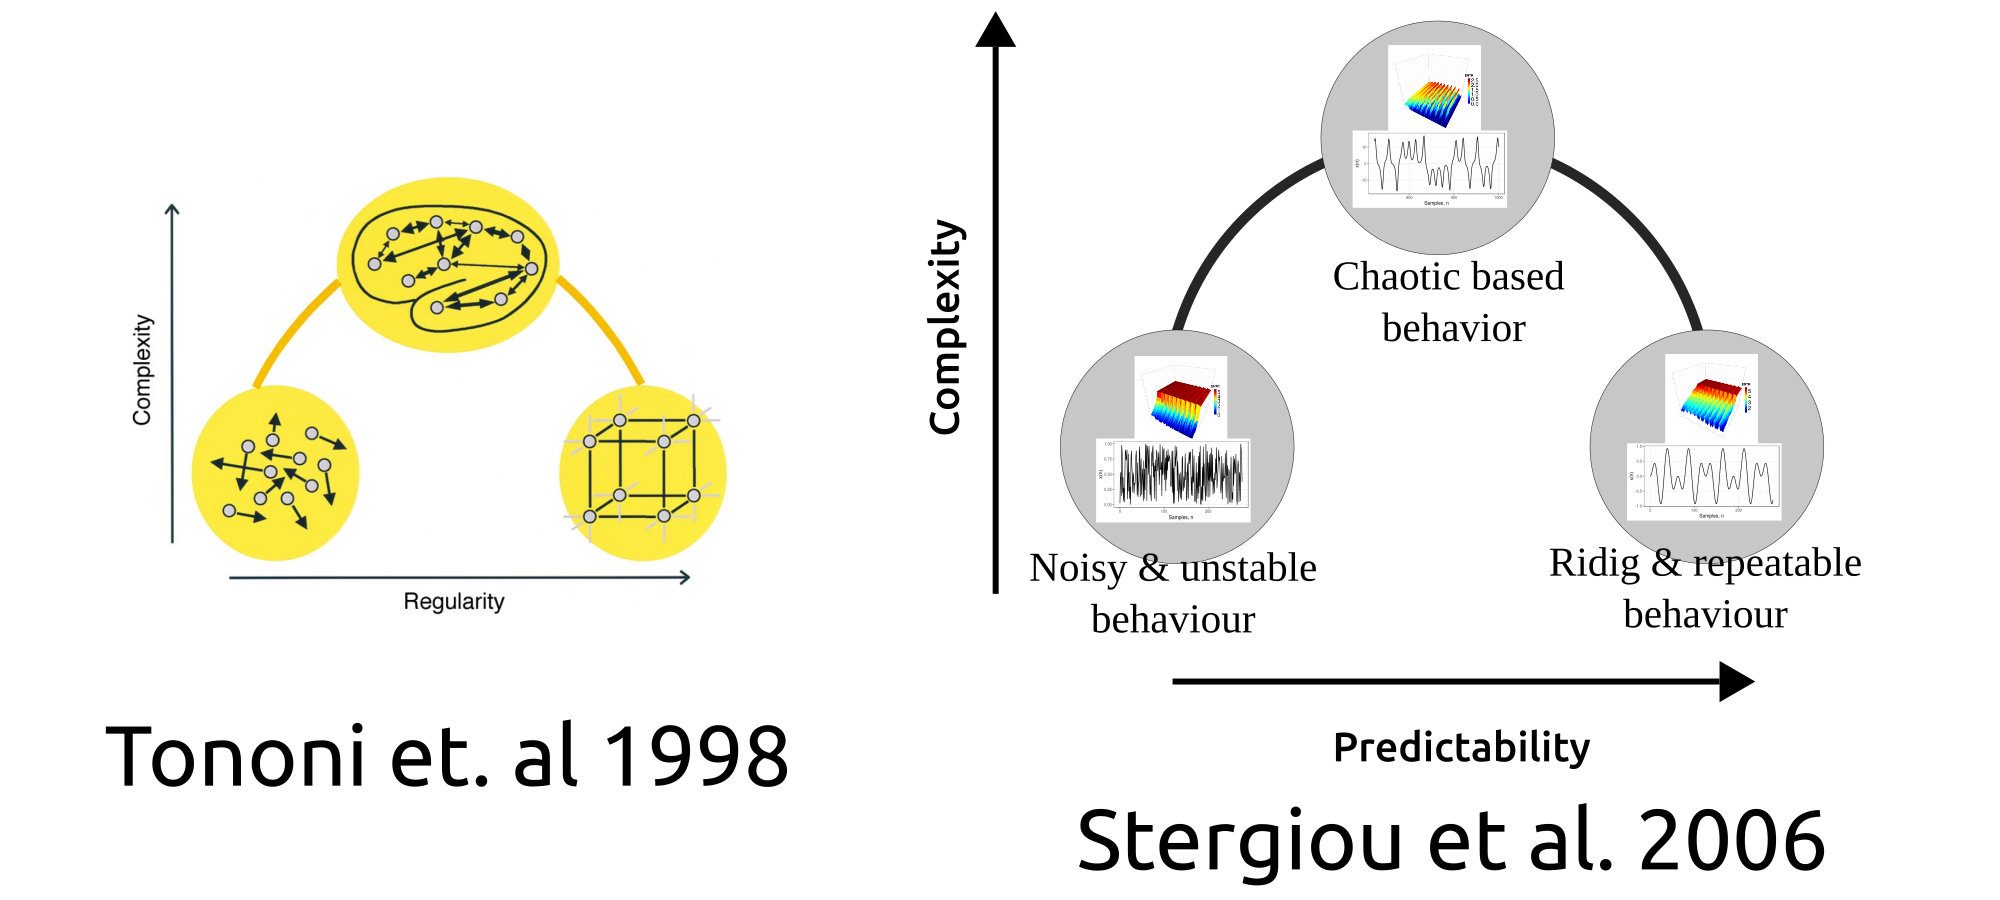
\includegraphics[width=0.95\linewidth]{./figs/modeling-movement-variability/versions/drawing-v00.png}
	%\caption{Theoretical Model of Optimal Movement Variability}
   \end{figure}
\end{frame}
}

